\section{Background}
For the background of this project, it is necessary to consider literature related to the following:
\begin{mylist}
  \item Mechanical design of existing sorting machines
  \item Existing Computer Vision systems for component identification
  \item Real-time Computer Vision architectures
\end{mylist}
\subsection{Mechanical Design}
\noindent
\textbf{Bowl Feeders} \\
In my research, I have discovered that most industrial sorting machines use a Vibratory Bowl Feeder (VBF) to feed components into the system;
as shown in Figure \ref*{fig:feeder}, the VBF consists of a bowl that vibrates coupled with a spring and electromagnet to feed components into the system.
The paper by \citet{nam2019design} explores the optimal design of a VBF for USB keycaps, by attempting to identify the ideal parameters for the structure of the bowl,
sorting track, mounting adapter, and suspension system. The paper also uses modal analysis to determine the natural frequencies of the system, and uses this to
avoid resonant conditions that might cause inefficient or erratic operation.

This paper is useful as it provides a comprehsive overview of the design of a VBF, and provides a good starting point for the design of the VBF for in the future
when the project is extended to include a VBF for fully autonomous sorting. The paper also provides a good overview of the design considerations for the VBF, and so can be used as a reference
during the design process.

Additionally, \citet{REINHART2010191} delves into the mathematical modelling of a VBF, focusing more on the overall performance of the VBF rather than efficiency, and \citet{ForceAnalysisofVibratoryBowlFeeder}
provides a good overview of the forces involved in the operation of a VBF, stengthening the basis for its design and viability.

The paper by \citet{zhang2019design} outlines a sorting system for vials, and does not make use of a VBF, instead opting for a turntable design that mechanically orientates the vials. It primarily operates
by using a design that is specific to the geometry of the vials, and so is not applicable to this project, however it does provide a good insight into the design of a sorting system.

It seems conclusive that a VBF is the most viable option for the feeding mechanism of the sorting system, and so the design of the VBF will be based on the research outlined above.

\begin{figure*}[t]
  \begin{minipage}[t]{0.45\textwidth}
    \centering
    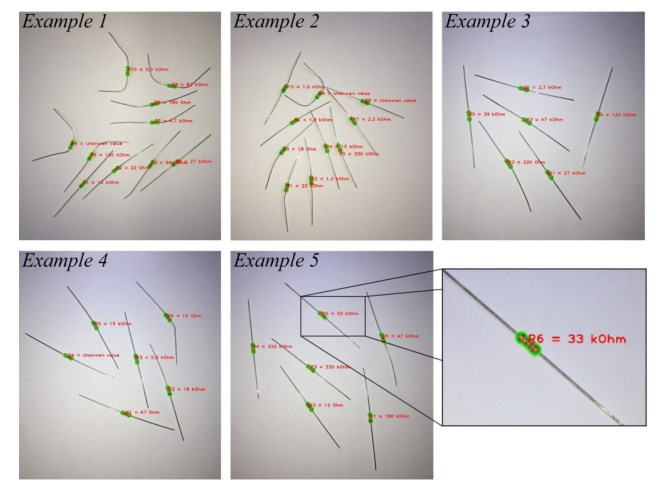
\includegraphics[width=\textwidth]{imgs/articles/resistordata.jpg}
    \caption{Resistor Test Set \cite{8939034}}
    \label{fig:resistordata}
  \end{minipage}
\end{figure*}

\noindent
\textbf{Transport Mechanisms} \\
The paper by \citet{Dhenge2013MechanicalNS} depicts a conveyer belt system that transports Nuts and Bolts to a computer vision system for identification, which aligns with the goals of the project. 
The hardware prototype is shown in Figure \ref*{fig:conveyer}, and a down-facing webcam is used to capture images of the components as they pass by. The webcam uses Principle Component Analysis (PCA) to identify the components,
which will be discussed in the next section.

The components then seperate into two chutes, one for Nuts and one for Bolts, using a stepper motor, which may be useful for the future design of the sorting system.
Additionally, the approach taken by the paper \citet{eggsorting} to sort Philippine table eggs also features a similiar conveyer belt system, down facing camera and an arm to sort the eggs into different categories. 

The approaches taken here are similiar to industrial sorting systems that I have come across in videos during my research; and this approach seems to answer two major design questions for the project, namely
how to transport the components to the computer vision system, and how to transport the components from the computer vision system to the sorting system.

The use of a converyer belt system is obvious, but the concept of having the camera facing down at the components is not one that I had considered initially, as for the first stage I wanted the system to be semi-autonomous;
having the camera face-up allows the user to simply place the component on a plate that was directly above the camera, and the component would be immediately identified. Having the camera face down
would block the user's view of the component, which would be a major inconvenience. However, it seems that this would be the most viable approach for the future of the project.

\begin{figure*}[t]
  \begin{minipage}[t]{0.45\textwidth}
    \centering
    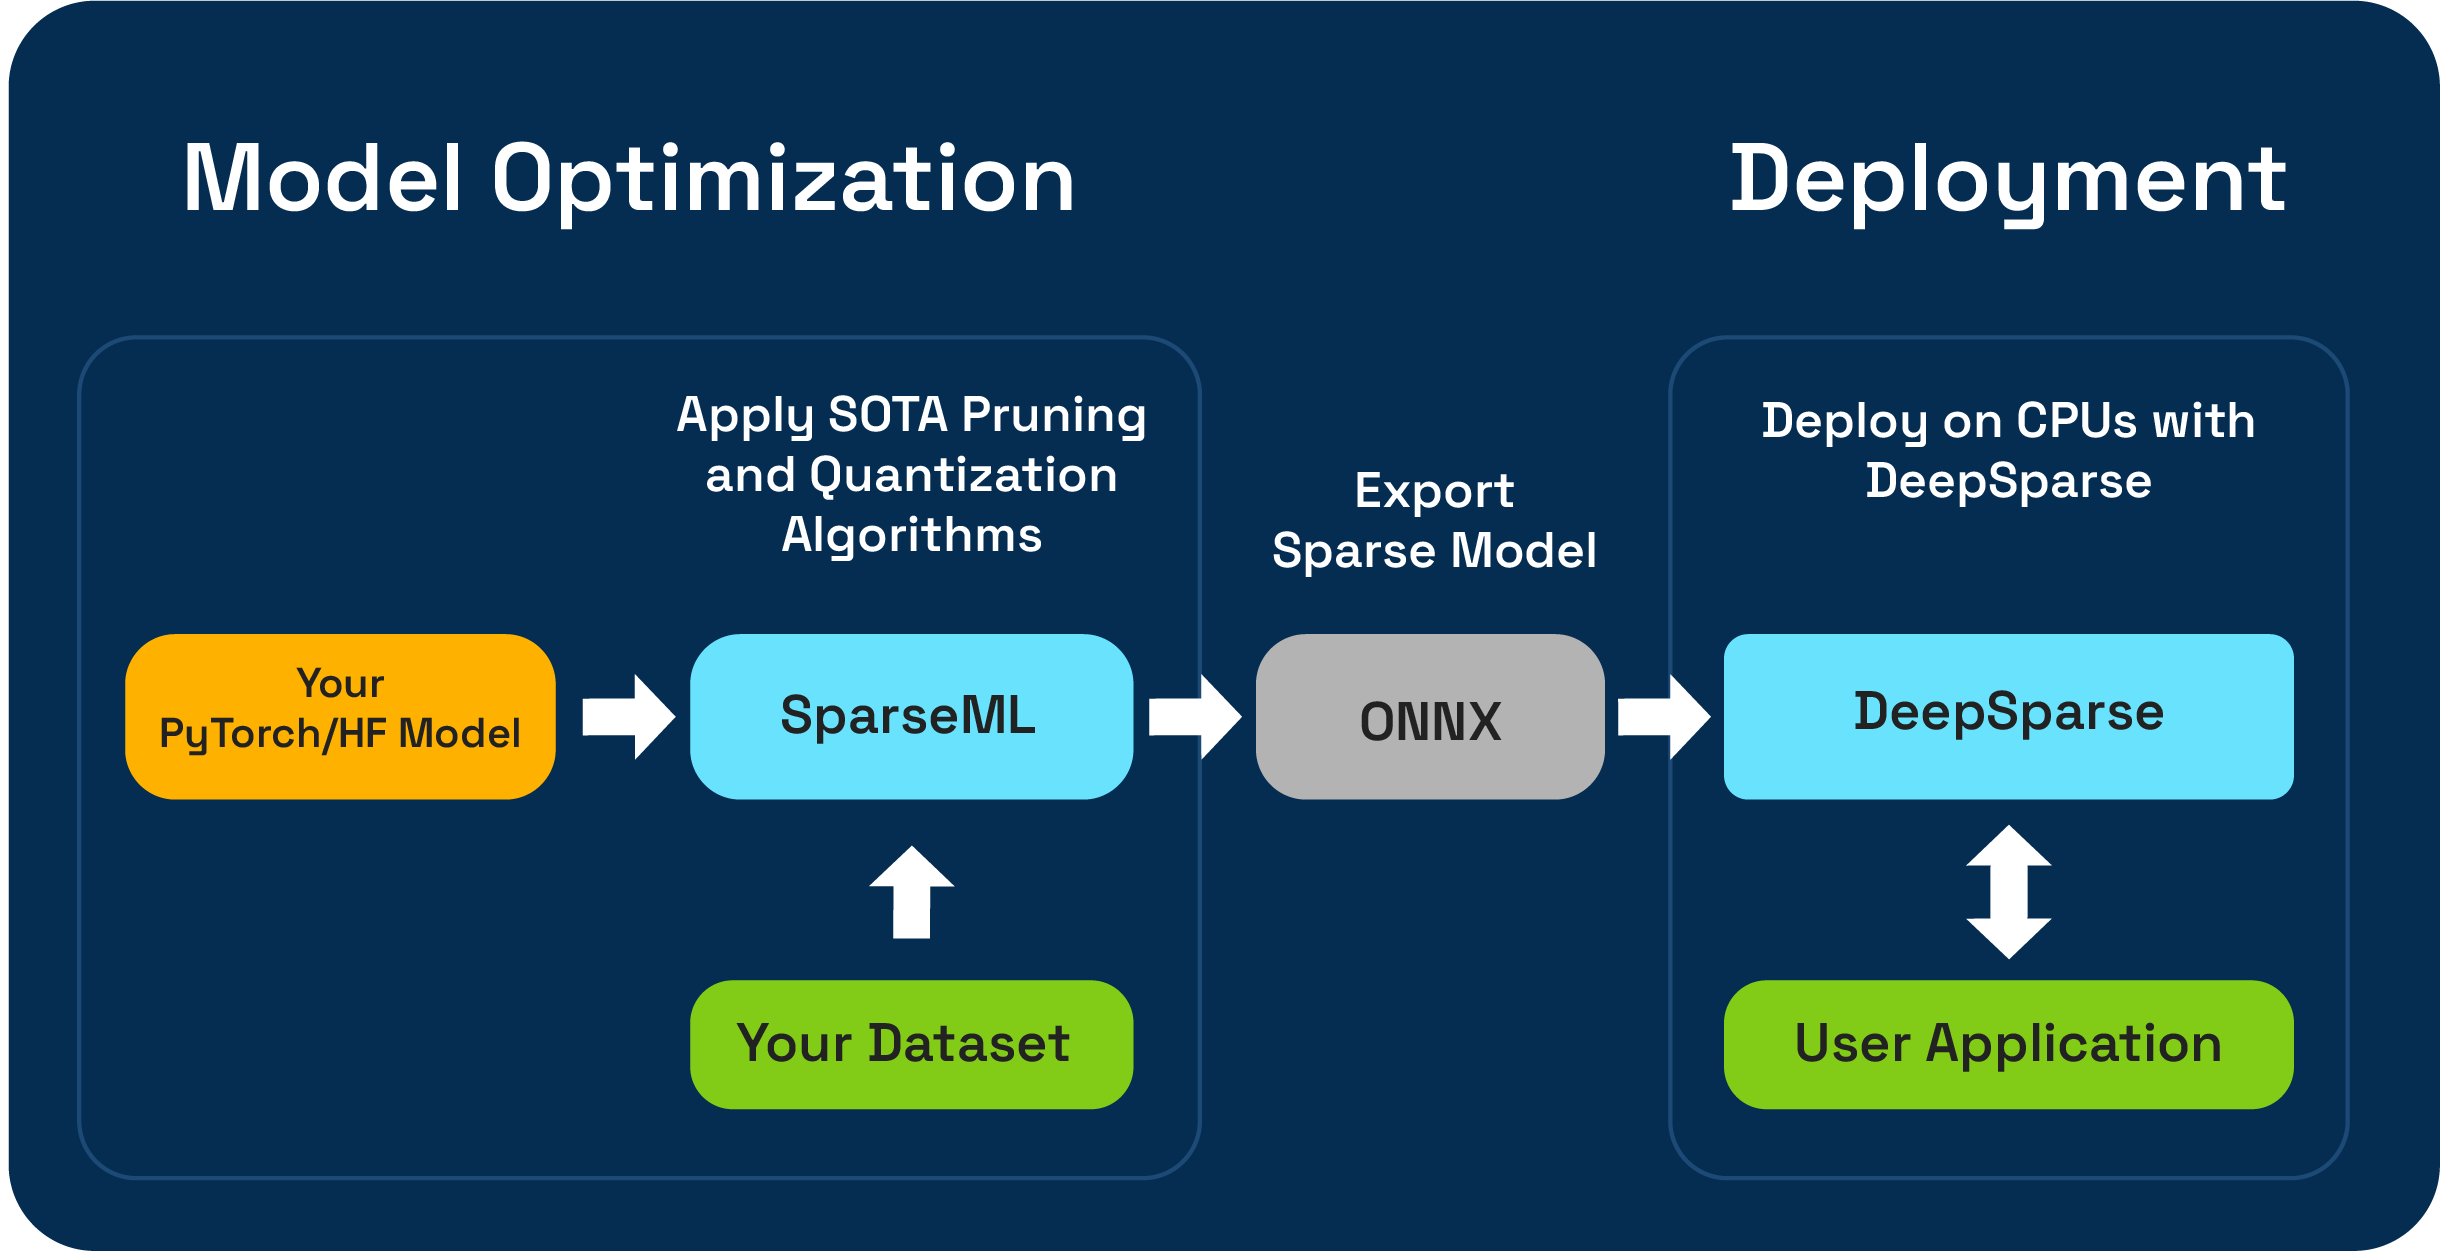
\includegraphics[width=\textwidth]{imgs/articles/sparseml-workflow.png}
    \caption{SparseML Pipeline \cite{sparseml}}
  \end{minipage}
  \hfill
  \begin{minipage}[t]{0.45\textwidth}
      \centering
      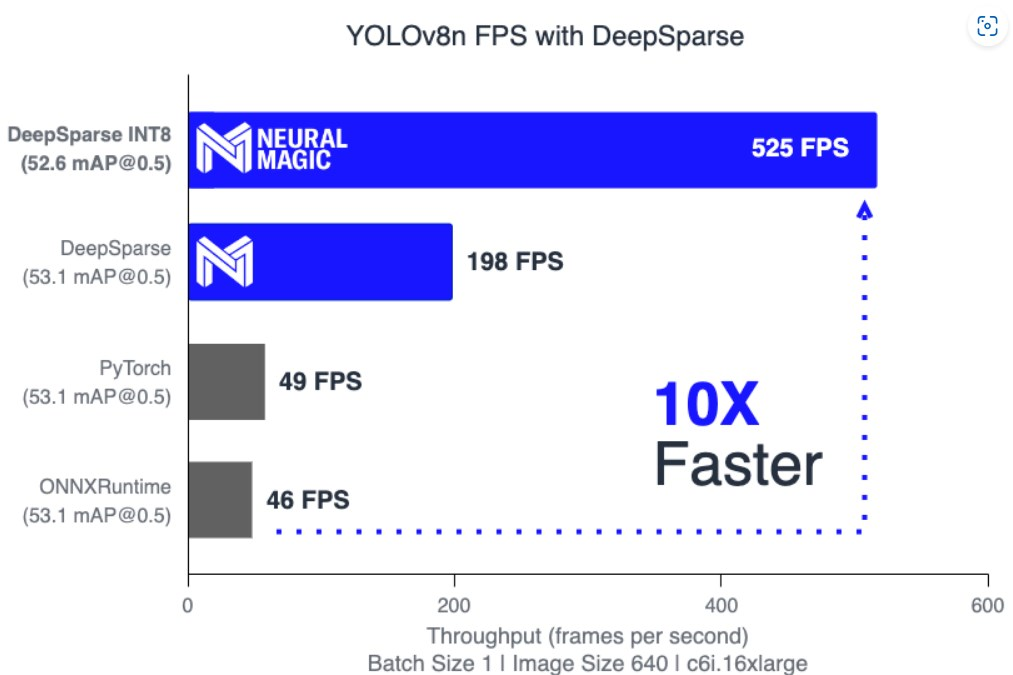
\includegraphics[width=\textwidth]{imgs/articles/yoloperf.jpg}
      \caption{DeepSparse Performance \cite{neuralmagic}}
      \end{minipage}
\end{figure*}
\subsection{Existing Computer Vision Systems}
A range of Computer Vision systems have been explored in the literature, ranging from PCA (Principle Component Analysis) \citet{Dhenge2013MechanicalNS} to more modern Computer Vision techniques \citet{Xu2020,s22239079}. However, given the rate of advancement of Computer Vision
techniques, the techniques used in the literature reflect the state of the art at the time of writing, and so are not necessarily the most viable current techniques for the project, but they inspire novel approaches to the problem of component identification.

PCA with ANN (Artificial Neural Network) as used by \citet{Dhenge2013MechanicalNS} is a relatively simple but outdated statistical technique that was successful in identifying nuts and bolts, which are very distinct components. 
In this paper, PCA is used as a feature extractor and then fed directly into, though not explicitly mentioned, an FCL (Fully Connected Layer), as the classifier. Although a valid approach, CNNs (Convolutional Neural Networks) have been shown to be much more
effective at feature extraction, and do not "have the problem of low recall and accuracy", as mentioned by \citet{Xu2020}, that PCA may suffer from, and so this approach is not viable for the project. 

The paper by \citet{Xu2020} use the SqueezeNet CNN architecture to identify 22 different subcategories of electronic components, specifically resistors, capacitors, and inductors, and acheives a True Positive Rate (TPR) of 99.999\% with only a 2.67ms average inference time on a 
GTX 1050 2GB GPU, released in 2016, an impressive result. This informs the design of the Computer Vision system, as it shows that a CNN is a viable approach to the problem of component identification.

The paper by \citet{8939034} dicuss the use of SVM to characterise resistors, by identifying the resistor's centroid (centre of mass), determining the resistor's orientation, and then analysing the bands to determine the resistor's value.
This is directly applicable to the project, as it is a viable approach to identifying resistors, which is very distinct from other components, given the colour bands. The paper's novel approach to identifying the resistor values allows it to achieve high accuracy (86\%, however
the test images used are resistors that are positioned far away from the camera, as shown in Figure \ref*{fig:resistordata}, and so the bands are very small, which will not be the case in the project's vision system, so the accuracy will likely be higher) which makes it very promising for the project,
and will inform the design of the Computer Vision system.


\subsection{Real-time Computer Vision Architectures}
For the problem of component identification, the Computer Vision system must be able to identify components in real-time, as the components will be moving on a conveyer belt, captured using
a camera facing down at the components. This means that the Computer Vision system must be able to identify components in a single frame, and not require multiple frames to identify a component.
As I envision the system to be self-contained, it must also be able to run on the Raspberry Pi 4, which has a 1.5GHz quad-core 64-bit ARM Cortex-A72 CPU, and 2GB of RAM. 
The system will also display a camera feed to the user, and so the Computer Vision system must be able to run in real-time alongside the camera feed.

This requires the Computer Vision system to be both computationally efficient and accurate, which is a difficult balance to strike.

For the explicit purpose of identifying electronic components, the paper by \citet{s22239079} compares a range of different object detection architectures, including YOLOv3, YOLOv4 and Faster SqueezeNet, with YOLOv4 achieving a mAP (mean Average Precision) of 98.6\%.

YOLO (You Only Look Once) is a real-time object detection architecture, that is used very commonly in Computer Vision applications, and has been shown to be very effective at identifying objects in real-time \citet{yolo}. It makes
use of a single CNN that takes in an image and outputs a list of bounding boxes and class probabilities for each bounding box. This is in contrast to other object detection architectures, such as R-CNN, which uses a CNN to propose regions of interest, and then uses a second CNN to classify the regions of interest.

Other papers like \citet{Guo2021} also comment on YOLOv4's effectiveness at identifying electronic components, achieving 93.94\% mAP on a dataset of 20 different components, and the paper also comments
on YOLOv4's ability to run in real-time, acheiving 67 FPS, albeit on a powerful NVIDIA TITAN Xp GPU. For the Raspberry Pi 3B, the paper by \citet{9166199} has shown to run YOLOv3 at a very low 1 FPS,
with an IoU (Intersection over Union) accuracy of 86.7\%, which is very low. 

However, efforts made by Neural Magic \cite{neuralmagic} in the optimisation of YOLOv5 and YOLOv8 show performance improvements of up to 10x on CPUs, through their open-source 
optimisation toolkit SparseML \cite{sparseml} and CPU inferencing runtime, DeepSparse \cite{deepsparse}; a very promising result.

Additionally, the YOLO architecture is one that I will likely come across in my modules Deep Learning COMP70010 and Machine Learning COMP70014, which will serve
to deepen my understanding of the architecture and allow me to make more informed design decisions.

As such, the purposes of this project, I will be using the YOLOv8 architecture.

